\documentclass[11pt]{article}
\usepackage{authblk}
\usepackage{graphicx}
\usepackage{amsmath,amsfonts,amssymb,amsthm, physics,mathrsfs}
\usepackage[margin=1in]{geometry}
\usepackage[colorlinks]{hyperref}
\usepackage{xcolor}
\usepackage{subfiles}
\usepackage{subcaption}

\newcommand{\C}{{\mathbb{C}}}
\newcommand{\F}{{\mathbb{F}}}
\newcommand{\R}{{\mathbb{R}}}
\newcommand{\Z}{{\mathbb{Z}}}

\theoremstyle{plain}
\newtheorem{theorem}{Theorem}[section]
\newtheorem{lemma}[theorem]{Lemma}
\newtheorem{corollary}[theorem]{Corollary}
\newtheorem{definition}[theorem]{Definition}



\newcommand{\eq}[1]{(\ref{eq:#1})}
\renewcommand{\sec}[1]{Section~\ref{sec:#1}}

\begin{document}

%%%%%%%%%%%%%%%%%%%%%%%%%%%%%%%%%%%%%%%%%%%%%%%%%%%%%%%%%%%%%%%%%%%%%%%%%%%%%%

\title{Exploring Graph Dynamics and Transport Properties with Staggered Quantum Walks}

\author[1]{B. Chagas}
\author[2]{W. S. Dias}
\author[3]{J. Santos}



\affil[1]{Mastercard, Dublin, Ireland}
\affil[2]{Instituto de Física, Universidade Federal de Alagoas, 57072-900 Maceió, Alagoas, Brazil}
\affil[3]{Haslab, INESC TEC, Portugal}

\date{\today}
\maketitle

%%%%%%%%%%%%%%%%%%%%%%%%%%%%%%%%%%%%%%%%%%%%%%%%%%%%%%%%%%%%%%%%%%%%%%%%%%%%%%
\begin{abstract}
Quantum walks provide a versatile framework for quantum algorithms and
transport properties within graph-encoded structures. In this study, we
investigate the staggered quantum walk model, incorporating angle decoherence
and alterations in graph structure through tessellation. These modifications
may entail disruptions in connections or shifts in operator orders.
Additionally, we analyze various transport properties, including mean, standard
deviation, inverse participation ratio, and localization. Through computational
simulations, we shed light on the intricate interplay between quantum walk
dynamics and graph evolution, offering insights into the fundamental properties
of quantum systems and their potential applications in quantum computing and
transport phenomena.  
\end{abstract}

\section{Introduction} \label{intro}

The exploration of quantum walks, quantum analogs of random walks, has garnered
significant attention in both physics and computer science, mainly due to the
advancements in quantum computation. Unlike their classical counterparts,
quantum walks take advantage of quantum coherence, enabling interference
effects that lead to the ballistic spreading of the walker. This unique
characteristic has proven invaluable in various applications, from designing
quantum search algorithms~\cite{PhysRevA.67.052307,Portugal2018} and
implementing communication protocols~\cite{Shang_2018,8972594} to achieving
universal quantum
computation~\cite{PhysRevA.81.042330,doi:10.1126/science.1229957}. Moreover,
quantum walks are versatile tools for simulating diverse physical phenomena,
including quantum phase transitions~\cite{Cardano2016,PhysRevLett.122.020501},
interacting particles~\cite{PhysRevB.76.155124,doi:10.1126/science.1260364},
rogue waves~\cite{PhysRevA.106.012414,PhysRevA.108.062206}, and nonlinear
dynamics~\cite{PhysRevA.75.062333,PhysRevA.101.023802}. Their effectiveness in
these applications underscores their potential as powerful environments for
developing quantum algorithms and intuitive frameworks for studying and
exploring quantum systems. However, harnessing the full capabilities of quantum
walks necessitates a profound understanding of the underlying dynamics,
particularly in designing and controlling these quantum processes over extended
periods.

Quantum walks are generally categorized into continuous- and discrete-time
versions, each exhibiting distinct characteristics. Continuous-time quantum
walks involve a unitary time evolution dictated by a Hamiltonian, providing the
walker's dynamics in continuous time within a discrete spatial
framework~\cite{PhysRevA.58.915}. In discrete-time quantum walks, the evolution
of the walker occurs in discrete steps, often relying on internal degrees of
freedom and sequential application of quantum operators to dictate its
dynamics. Two of the most well-known versions are the
coined~\cite{PhysRevA.48.1687} and the Szegedy~\cite{1366222} models. The
essential feature of the coined quantum walk lies in utilizing an internal
state to dictate the potential directions the particle may traverse. During
each step, the walker undergoes an operation involving the sequential
application of the coin operator, which controls state changes, and the shift
operator, which determines the feasible directions for particle movement. On
the other hand, Szegedy's quantum walk arises as a coinless quantization of
classical Markov chains following a transition matrix. This model combines
evolution and mixing operators through a unitary operation, providing a
versatile framework for quantum walk dynamics.

Staggered quantum walks represent a recent approach in discrete-time quantum
walks, offering a distinctive framework for investigating quantum dynamics on
graph structures~\cite{PhysRevA.93.062335,Portugal2016}. Unlike traditional
quantum walks, which proceed straightforwardly from one vertex to another,
staggered quantum walks introduce a partitioning scheme that divides arbitrary
graphs into tessellations. Such a tessellation-based approach provides a
structured framework for the evolution of quantum states, enabling the
exploration of complex graph structures with enhanced versatility and
precision~\cite{PhysRevA.98.052310,PhysRevA.98.012123}.  This model encompasses
a substantial portion of the subclass of discrete-time quantum walks, including
the coined and Szegedy's
models~\cite{Portugal2016,Portugal2016_1,PhysRevA.95.012328}.

Recent advancements have introduced extensions enabling physical realizations
of quantum walk dynamics using time-independent
Hamiltonians~\cite{PhysRevA.95.012328,PhysRevB.95.144506}, presenting exciting
opportunities for investigating quantum phenomena in well-controlled
experimental setups. However, it's essential to acknowledge that implementing
quantum systems is prone to decoherence, which can significantly impact the
performance of quantum
walks~\cite{KENDON_2007,PhysRevA.103.042213,PhysRevLett.104.153602,PhysRevLett.106.180403}.
Therefore, understanding how decoherence influences the transition from quantum
to other regimes is paramount and requires further exploration, particularly in
staggered quantum walks. The effect of breaking polygons and vertices has been
investigated on a two-dimensional grid of 4-cliques, revealing a loss of
quantum behavior~\cite{PhysRevA.105.032452}. Furthermore, the authors have
shown that resilience against decoherence can be improved by expanding the
intersection of tessellations within the graph. Considering that fault-tolerant
architectures are constructed based on a thorough understanding of each
potential component, we explore here the inhomogeneity in tessellations as the
main agent affecting the staggered quantum walk dynamics. 


\section{Staggered Quantum Walk Model}
\subfile{Sections/Sec2/staggeredQW}

\section{Computational Simulations}

\begin{itemize}
    \item Figure 1 - Temporal evolution of the standard deviation and return
        probability, considering the scenario without disorder and disordered.
        Well-known results for the case without disorder. With disorder, we
        must find a standard deviation saturating at a fixed value after some
        time of evolution. The return probability must also saturate at a
        finite value.

    \item Figure 2 - Probability distribution. We can evaluate the distribution
        in the first stages of temporal evolution and the scenario where the
        localization (saturation of $\sigma$) is already well established. I
        believe that the exponentially localized profile will be dominant in
        this last scenario.

    \item Figure 3 - Evaluate the initial transient time as a function of the
        disorder degree, considering the standard deviation. In figure (a), we
        can show examples, and in figure (b), a graph of ``saturation time" vs.
        ``disorder degree." I believe that the saturation time is inversely
        proportional to the disorder width.

    \item Figure 4 - Considering using a certain tessellation in all previous
        figures, we can try to generalize the study, considering other
        tessellation relationships (equivalent to changing the $\theta$).
        Another possibility is to apply these considerations to a well-known
        algorithm, such as search or hitting time. In the search, unless I'm
        mistaken, there is an optimal value to retrieve the optimal number of
        steps O($\sqrt{N\ln N}$) and the success probability O($1/ \ln{N} $).
        How does our model impact this performance? Anyway, there are two
        possible itineraries to conclude our article. What do you think is most
        viable?.

\end{itemize}




\bibliographystyle{acm}
\bibliography{biblio}

\clearpage

\section{Anotações}

Pessoal, acabo de ver os experimentos na seção seguinte. Pelo que pude entender, foi estabelecido $\theta=\pi/3$ em todos os cenários, entretanto, tive dificuldade em entender a diferença entre as configurações das figuras 5, 6, e 7. Entendi que a figura 4 considera um sistema sem desordem e possivelmente as outras possuem. Sobre este ponto, gostaria de salientar para o caso de sensibilidade e tempo de evolução. Possivelmente, nesta largura de desordem, precisaremos de 2000 steps ou mais para perceber uma influência efetiva. Outro ponto é sobre o número de amostras. Com $\approx 5$ amostras teremos um ensaio sobre o perfil do caminhante, bem como sua medida de desvio quadrático médio minimamente confiável. 


\clearpage

\section{Experimentos}
\subsection{Dinâmica Simples}
\begin{figure}[!h]
	\centering
	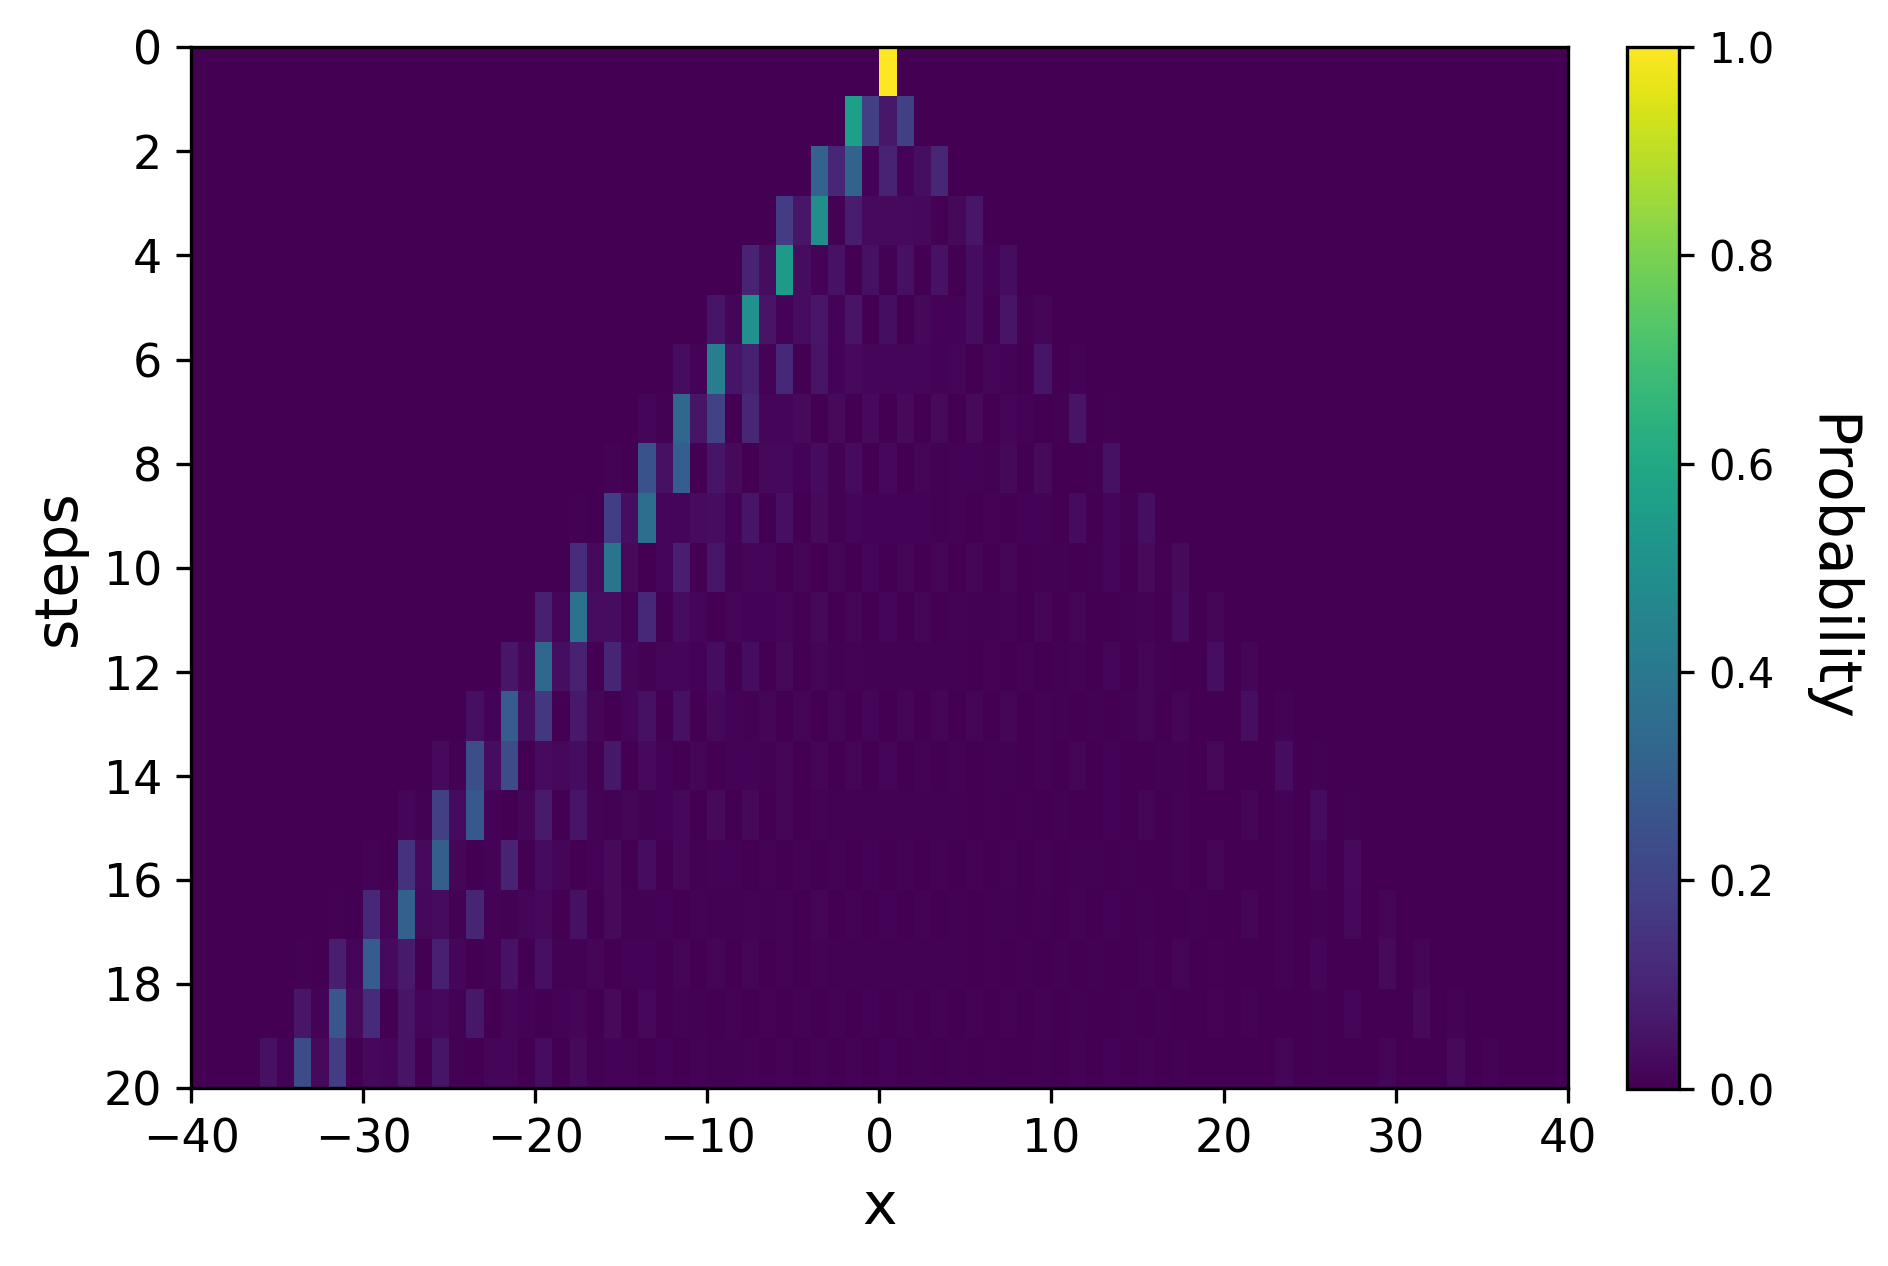
\includegraphics[scale=0.70]{img/Experiments/sqw_N121_t20_thetapi3-pi3_init0.png}
	\caption{Probability distribution for the staggered quantum walk on a line after 20 steps, with initial condition $\ket{\psi(0)}=\ket{50}$, and $\theta = \pi/3$} 
	\label{fig:stagQWSimulMultTheta}
\end{figure}\par


\begin{figure}[!h]
	\centering
	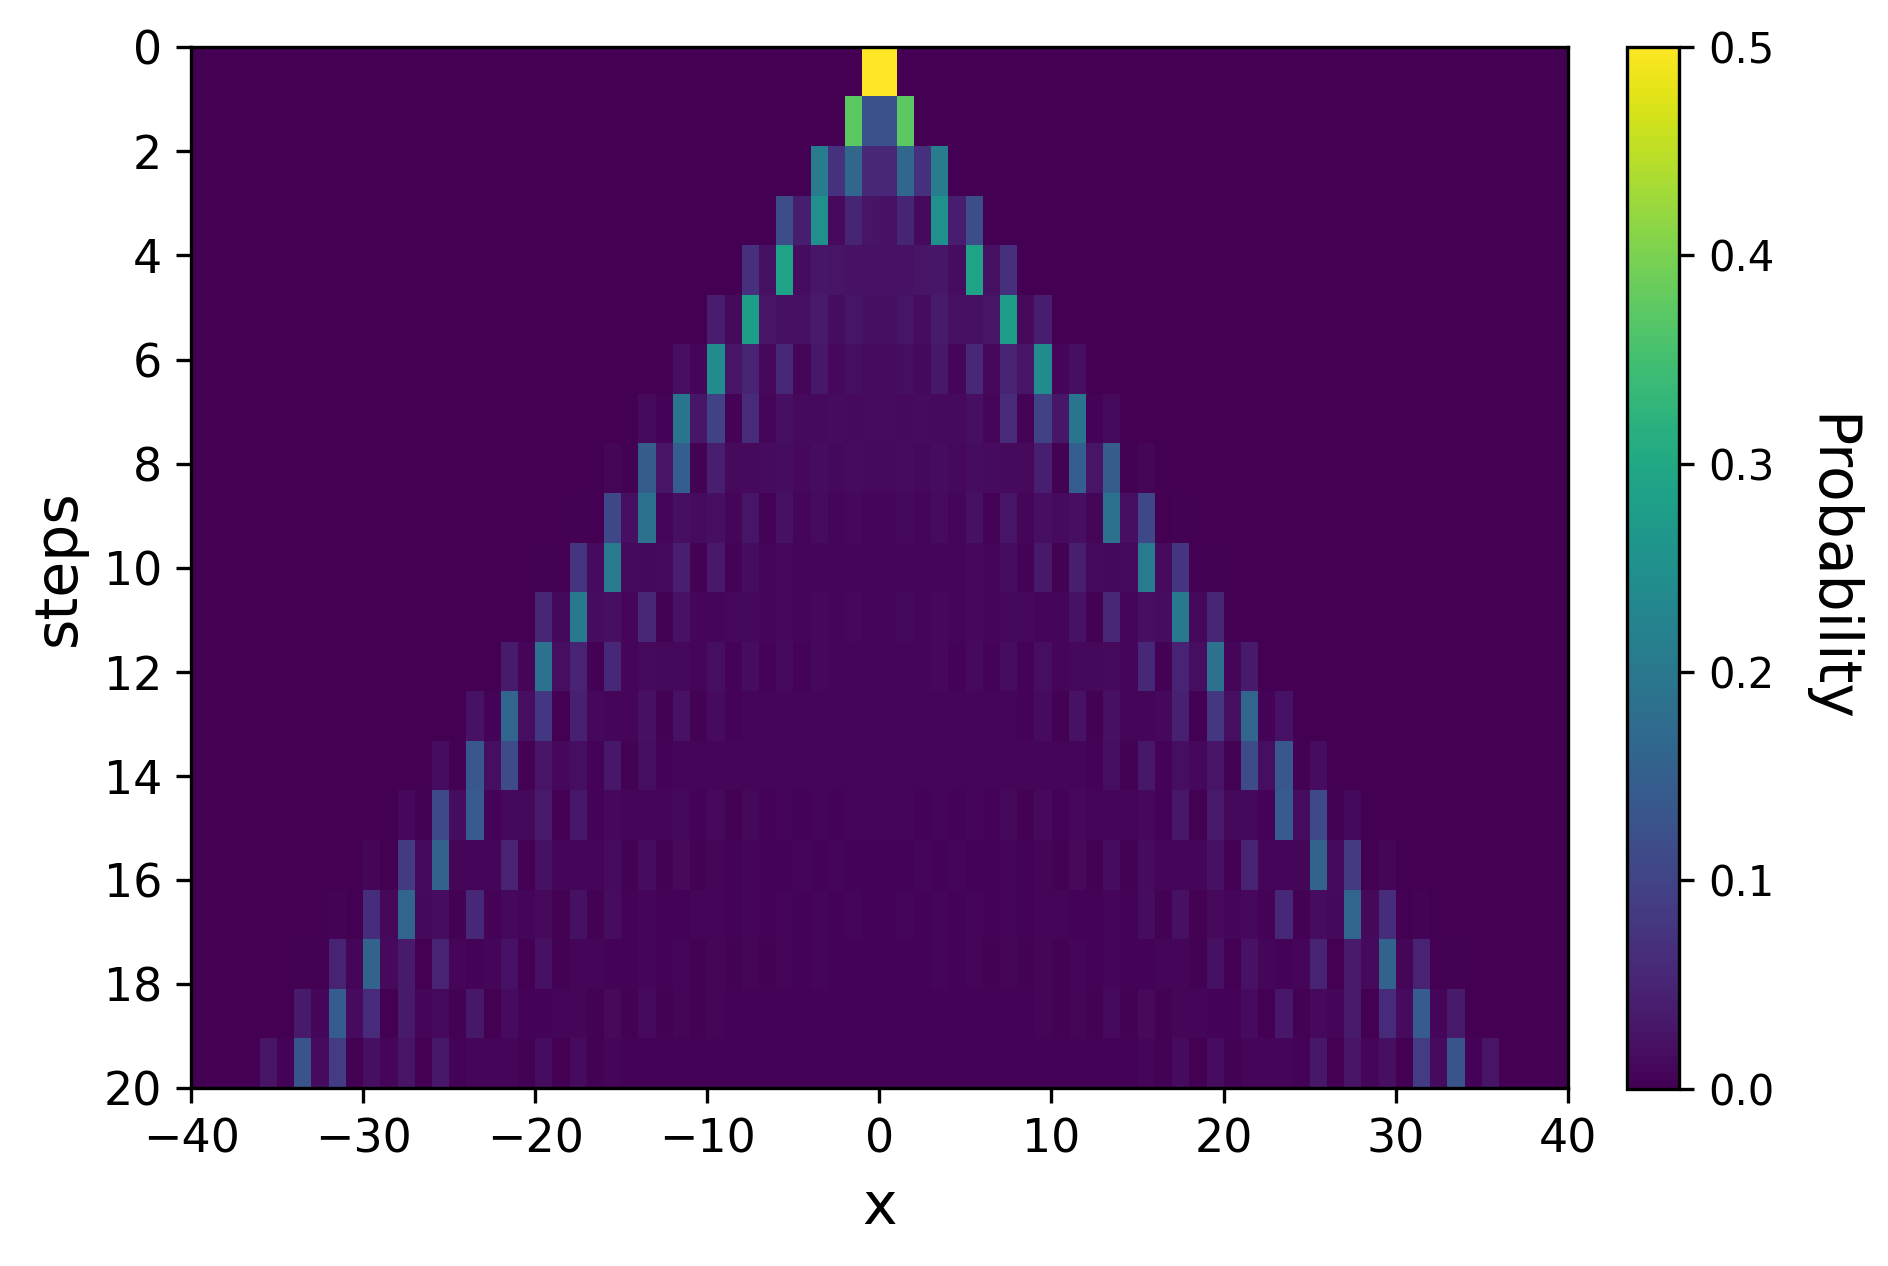
\includegraphics[scale=0.70]{img/Experiments/sqw_N121_t20_thetapi3-pi3_init0-1.png}
	\caption{Probability distribution for the staggered quantum walk on a line after 20 steps, with initial condition $\ket{\psi(0)}=\ket{50}$, and $\theta = \pi/3$, and angles with deviation of $0.4$} 
	\label{fig:stagQWSimulMultTheta}
\end{figure}\par

\begin{figure}[!h]
	\centering
	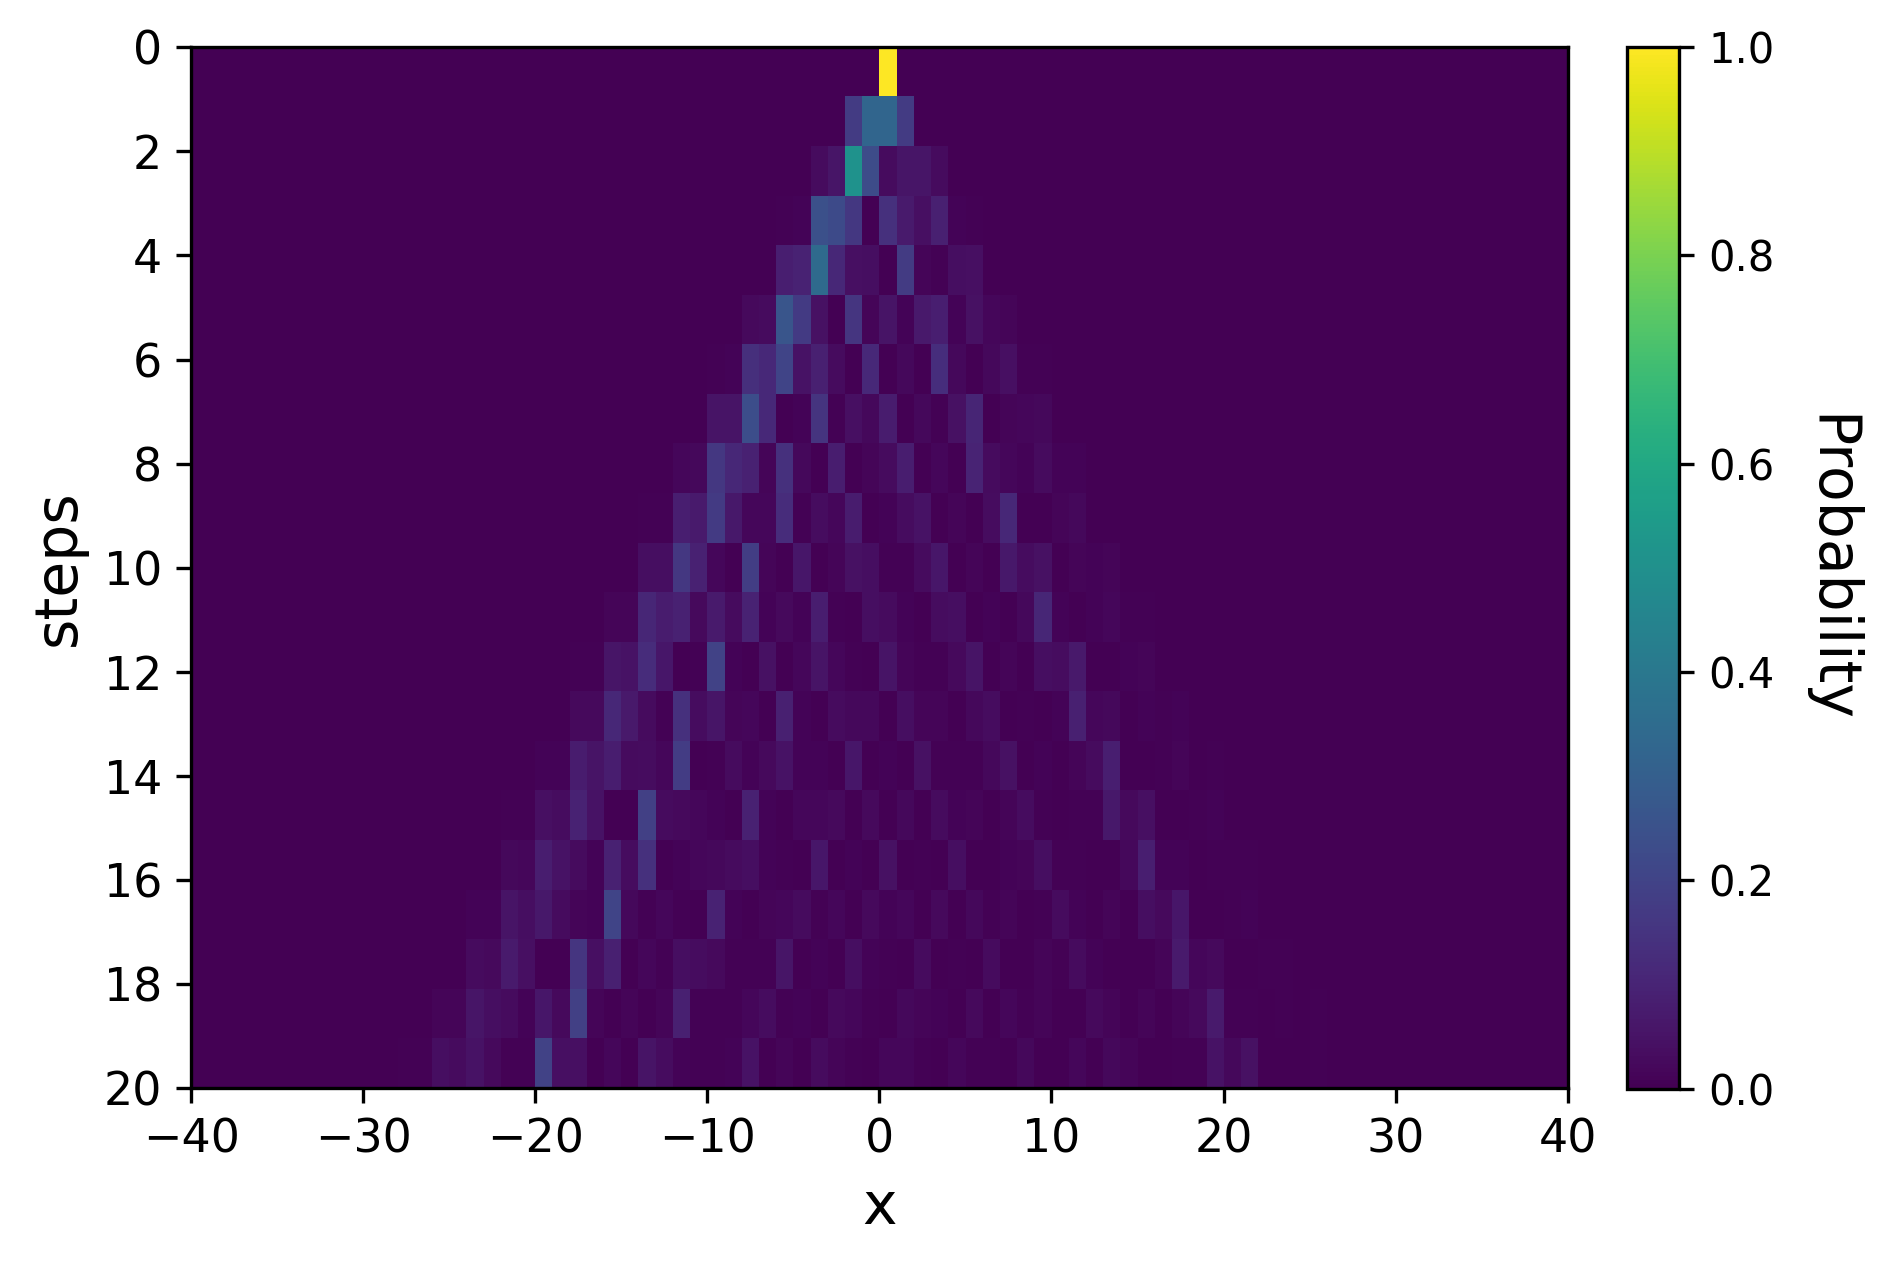
\includegraphics[scale=0.70]{img/Experiments/sqw_N121_t20_thetapi4-pi5_init0.png}
	\caption{Probability distribution for the staggered quantum walk on a line after 20 steps, with initial condition $\ket{\psi(0)}=\ket{50}$, and $\theta = \pi/3$, and angles with deviation of $0.4$} 
	\label{fig:stagQWSimulMultTheta}
\end{figure}\par

\begin{figure}[!h]
	\centering
	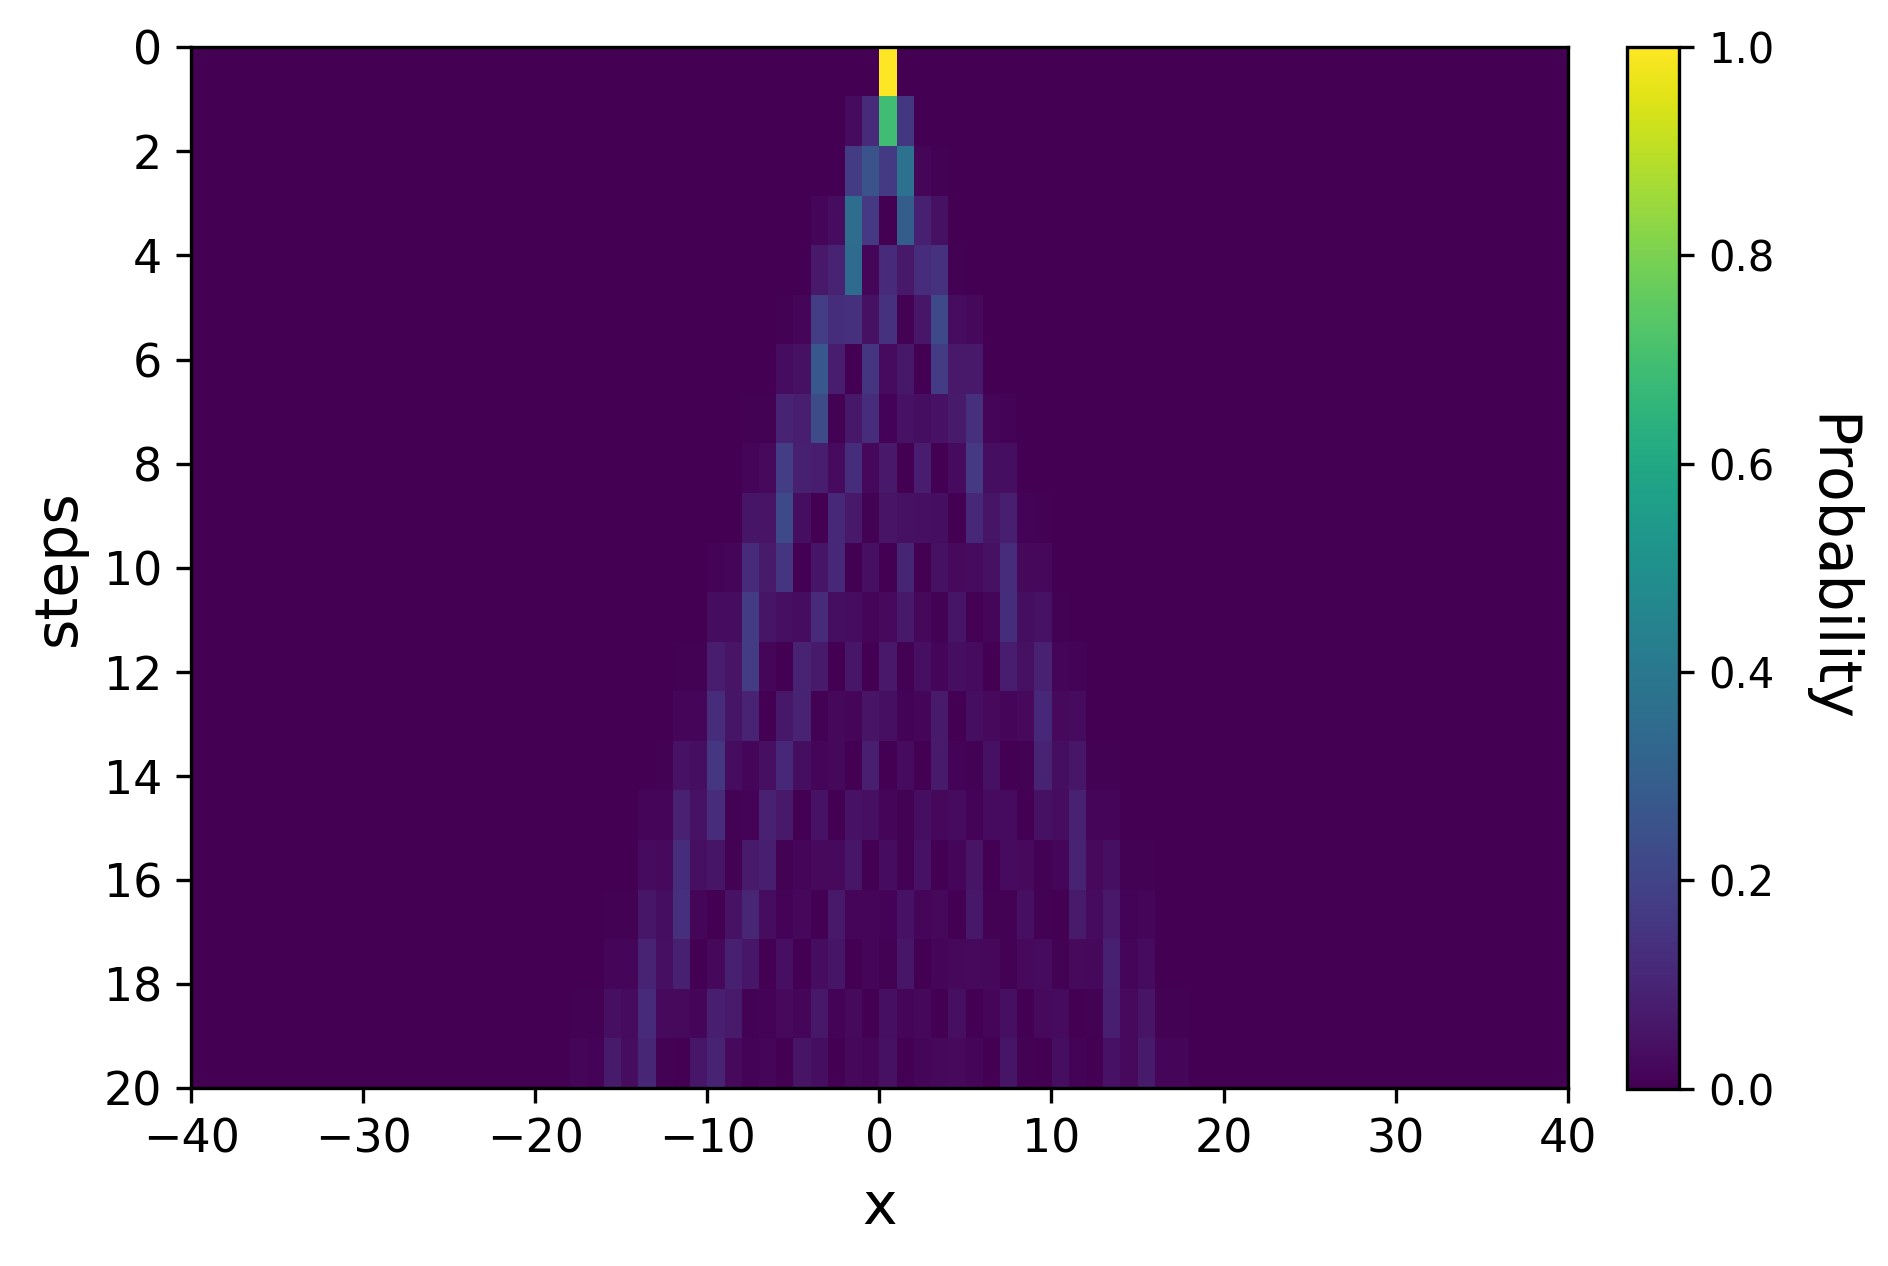
\includegraphics[scale=0.70]{img/Experiments/sqw_N121_t20_thetapi8-pi7_init0.png}
	\caption{Probability distribution for the staggered quantum walk on a line after 20 steps, with initial condition $\ket{\psi(0)}=\ket{50}$, and $\theta = \pi/3$, and angles with deviation of $0.4$} 
	\label{fig:stagQWSimulMultTheta}
\end{figure}\par

\end{document}
